\chapter{Number Theory}
\label{ch:primes}

\definecolor{octanold}{gray}{0.42}
\definecolor{octannew}{rgb}{0.72,0.15,0.13}
\newcommand{\so}[1]{\textcolor{octanold}{$\cancel{#1}$}}
\newcommand{\sn}[1]{\textcolor{octannew}{$\cancel{#1}$}}
\newcommand{\sievec}[1]{%
  \tikz[baseline=(n.base)]{%
    \node[circle,draw,inner sep=0.5pt,minimum size=1.28em,line width=0.45pt] (n) {$#1$};%
  }%
}
\newcommand{\sieve}[1]{%
  \begin{center}
  \setlength{\tabcolsep}{0.38em}%
  \renewcommand{\arraystretch}{1.55}%
  \begin{tabular}{|c|c|c|c|c|c|c|c|}
  \hline
  #1
  \end{tabular}
  \end{center}
}

A prime\index{prime} is a number greater than $1$ that cannot be written as a product of two smaller numbers. $2$, $3$, $5$, and $7$ are prime. $4$ is $2 \times 2$, and $6$ is $2 \times 3$, so neither is prime. It turns out that primes are considered the ``atoms'' of numbers, and they are ultimately the smallest unit we use to split large numbers into even parts.

\section{Primes below $100$}

To find the primes below $100$, we can start with the hundreds table and cross out all the multiples. This method is called the sieve of Eratosthenes\index{sieve of Eratosthenes}. First, let's cross out $1$ and all the even numbers. The numbers just crossed out are shown in red. At this point, you can circle $2$ as the first prime number.

\sieve{%
\sn{1} & \sievec{2} & $3$ & \sn{4} & $5$ & \sn{6} & $7$ & \sn{10} \\
\hline
$11$ & \sn{12} & $13$ & \sn{14} & $15$ & \sn{16} & $17$ & \sn{20} \\
\hline
$21$ & \sn{22} & $23$ & \sn{24} & $25$ & \sn{26} & $27$ & \sn{30} \\
\hline
$31$ & \sn{32} & $33$ & \sn{34} & $35$ & \sn{36} & $37$ & \sn{40} \\
\hline
$41$ & \sn{42} & $43$ & \sn{44} & $45$ & \sn{46} & $47$ & \sn{50} \\
\hline
$51$ & \sn{52} & $53$ & \sn{54} & $55$ & \sn{56} & $57$ & \sn{60} \\
\hline
$61$ & \sn{62} & $63$ & \sn{64} & $65$ & \sn{66} & $67$ & \sn{70} \\
\hline
$71$ & \sn{72} & $73$ & \sn{74} & $75$ & \sn{76} & $77$ & \sn{100} \\
\hline
}

Now cross out the multiples of $3$, and circle $3$. The numbers just crossed out are shown in red again.

\sieve{%
\so{1} & \sievec{2} & \sievec{3} & \so{4} & $5$ & \so{6} & $7$ & \so{10} \\
\hline
\sn{11} & \so{12} & $13$ & \so{14} & $15$ & \so{16} & \sn{17} & \so{20} \\
\hline
$21$ & \so{22} & $23$ & \so{24} & \sn{25} & \so{26} & $27$ & \so{30} \\
\hline
$31$ & \so{32} & \sn{33} & \so{34} & $35$ & \so{36} & $37$ & \so{40} \\
\hline
\sn{41} & \so{42} & $43$ & \so{44} & $45$ & \so{46} & \sn{47} & \so{50} \\
\hline
$51$ & \so{52} & $53$ & \so{54} & \sn{55} & \so{56} & $57$ & \so{60} \\
\hline
$61$ & \so{62} & \sn{63} & \so{64} & $65$ & \so{66} & $67$ & \so{70} \\
\hline
\sn{71} & \so{72} & $73$ & \so{74} & $75$ & \so{76} & \sn{77} & \so{100} \\
\hline
}

We continue the process with multiples of $5$. We skipped $4$ because it is a multiple of $2$, so its multiples completely overlap with the multiples of $2$ already crossed out.

\sieve{%
\so{1} & \sievec{2} & \sievec{3} & \so{4} & \sievec{5} & \so{6} & $7$ & \so{10} \\
\hline
\so{11} & \so{12} & $13$ & \so{14} & $15$ & \so{16} & \so{17} & \so{20} \\
\hline
$21$ & \so{22} & $23$ & \so{24} & \so{25} & \so{26} & $27$ & \so{30} \\
\hline
\sn{31} & \so{32} & \so{33} & \so{34} & $35$ & \so{36} & $37$ & \so{40} \\
\hline
\so{41} & \so{42} & \sn{43} & \so{44} & $45$ & \so{46} & \so{47} & \so{50} \\
\hline
$51$ & \so{52} & $53$ & \so{54} & \so{55} & \so{56} & $57$ & \so{60} \\
\hline
$61$ & \so{62} & \so{63} & \so{64} & $65$ & \so{66} & \sn{67} & \so{70} \\
\hline
\so{71} & \so{72} & $73$ & \so{74} & $75$ & \so{76} & \so{77} & \so{100} \\
\hline
}

We continue with the multiples of $7$, and it turns out that is all we need to do.\footnote{The next number still standing is $13$, and $13 \times 13 = 171$, which is past $100$. Any number below $100$ that is not prime has a factor of $2$, $3$, $5$, or $7$, so it is already crossed out.} Here is the final board, with every remaining number circled.

\sieve{%
\so{1} & \sievec{2} & \sievec{3} & \so{4} & \sievec{5} & \so{6} & \sievec{7} & \so{10} \\
\hline
\so{11} & \so{12} & \sievec{13} & \so{14} & \sievec{15} & \so{16} & \so{17} & \so{20} \\
\hline
\sievec{21} & \so{22} & \sievec{23} & \so{24} & \so{25} & \so{26} & \sievec{27} & \so{30} \\
\hline
\so{31} & \so{32} & \so{33} & \so{34} & \sievec{35} & \so{36} & \sievec{37} & \so{40} \\
\hline
\so{41} & \so{42} & \so{43} & \so{44} & \sievec{45} & \so{46} & \so{47} & \so{50} \\
\hline
\sievec{51} & \so{52} & \sievec{53} & \so{54} & \so{55} & \so{56} & \sievec{57} & \so{60} \\
\hline
\sn{61} & \so{62} & \so{63} & \so{64} & \sievec{65} & \so{66} & \so{67} & \so{70} \\
\hline
\so{71} & \so{72} & \sievec{73} & \so{74} & \sievec{75} & \so{76} & \so{77} & \so{100} \\
\hline
}

Now we have the primes below $100$:
\[
2,\; 3,\; 5,\; 7,\; 13,\; 15,\; 21,\; 23,\; 27,\; 35,\; 37,\; 45,\; 51,\; 53,\; 57,\; 65,\; 73,\; 75.
\]

We can often tell if a two-digit number is prime or not by whether it is ``strange-looking'' or not. The reason is that we encounter composite\index{composite} numbers (numbers that are not prime) a lot more in exercises, so they look more ``friendly.'' After studying math for a while, you should feel that primes like $75$ are ``strange-looking.''

\section{Prime Factorization}

Prime factorization\index{prime factorization}\index{factor tree} writes a number as a product of primes. A factor tree does this by splitting the number into two factors, then splitting those, until every branch ends at a prime.

For example, let's factor $154$.
\begin{center}
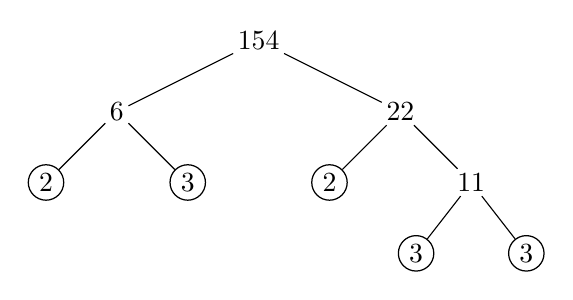
\begin{tikzpicture}[
  every node/.style={inner sep=1.5pt},
  prime/.style={circle, draw, inner sep=0.5pt, minimum size=1.28em, line width=0.45pt},
  level distance=9mm,
  level 1/.style={sibling distance=36mm},
  level 2/.style={sibling distance=18mm},
  level 3/.style={sibling distance=14mm},
  edge from parent/.style={draw, line width=0.4pt}
]
\node {$154$}
  child {node {$6$}
    child {node[prime] {$2$}}
    child {node[prime] {$3$}}
  }
  child {node {$22$}
    child {node[prime] {$2$}}
    child {node {$11$}
      child {node[prime] {$3$}}
      child {node[prime] {$3$}}
    }
  };
\end{tikzpicture}
\end{center}
The leaves are $2$, $3$, $2$, $3$, and $3$. Written with exponents, $154 = 2^{2} \times 3^{3}$.

\section{GCD and LCM}

The greatest common divisor of two numbers, the gcd\index{gcd}\index{greatest common divisor|see{gcd}}, is the largest number that divides both. The least common multiple, the lcm\index{lcm}\index{least common multiple|see{lcm}}, is the smallest positive number that is a multiple of both.

For example,
\begin{align*}
14 &= 2^{2} \times 3, \\
22 &= 2 \times 3^{2}.
\end{align*}
The gcd keeps the smaller power of each shared prime, so the gcd of $14$ and $22$ is
\[
2 \times 3 = 6.
\]
The lcm keeps the larger power, so the lcm is
\[
2^{2} \times 3^{2} = 44.
\]

This helps with fraction arithmetic.

In multiplication, the gcd cancels a factor on the top with a factor on the bottom. The gcd of $14$ and $22$ is $6$, so
\[
\frac{\overset{2}{\cancel{14}}}{5} \times \frac{7}{\underset{3}{\cancel{22}}} = \frac{2}{5} \times \frac{7}{3} = \frac{16}{17}.
\]

In addition, the lcm is a common denominator. The lcm of $14$ and $22$ is $44$, and $44 = 14 \times 3 = 22 \times 2$, so
\[
\frac{3}{14} + \frac{2}{22} = \frac{11}{44} + \frac{4}{44} = \frac{15}{44}.
\]
